% small.tex
\documentclass{beamer}
\usetheme{Boadilla}
\setbeamertemplate{blocks}[rounded][shadow=false] 

\usepackage{subfig}
\usepackage{multirow}
\usepackage{amsmath}
\usepackage{mathtools}
\usepackage{listings}
\usepackage{color}
\usepackage{natbib}
\usepackage{bm}
\usepackage{verbatim}
 
\definecolor{dkgreen}{rgb}{0,0.6,0}
\definecolor{gray}{rgb}{0.5,0.5,0.5}
\definecolor{mauve}{rgb}{0.58,0,0.82}

\lstset{ %
  language=Python,                % the language of the code
  basicstyle=\footnotesize,           % the size of the fonts that are used for the code
  %numbers=left,                   % where to put the line-numbers
  %numberstyle=\tiny\color{gray},  % the style that is used for the line-numbers
  %stepnumber=2,                   % the step between two line-numbers. If it's 1, each line 
                                  % will be numbered
  %numbersep=5pt,                  % how far the line-numbers are from the code
  %backgroundcolor=\color{white},      % choose the background color. You must add \usepackage{color}
  showspaces=false,               % show spaces adding particular underscores
  showstringspaces=false,         % underline spaces within strings
  showtabs=false,                 % show tabs within strings adding particular underscores
  %frame=single,                   % adds a frame around the code
  rulecolor=\color{black},        % if not set, the frame-color may be changed on line-breaks within not-black text (e.g. commens (green here))
  tabsize=2,                      % sets default tabsize to 2 spaces
  captionpos=b,                   % sets the caption-position to bottom
  breaklines=true,                % sets automatic line breaking
  breakatwhitespace=false,        % sets if automatic breaks should only happen at whitespace
  title=\lstname,                   % show the filename of files included with \lstinputlisting;
                                  % also try caption instead of title
  keywordstyle=\color{blue},          % keyword style
  commentstyle=\color{dkgreen},       % comment style
  stringstyle=\color{mauve},         % string literal style
  escapeinside={\%*}{*)},            % if you want to add a comment within your code
  morekeywords={dynamic, string}               % if you want to add more keywords to the set
}


\AtBeginSection[]
{
%    \begin{frame}
%        \frametitle{Table of Contents}
%        \tableofcontents[currentsection]
%    \end{frame}
}


%About me
\author{Wesley Brooks} 
\title[Lit review]{The literature on GWR}
%\subtitle{sub} 
\institute{UW-Madison} 

\begin{document}

    %Title slide
    \begin{frame}
        \titlepage
    \end{frame}


    %Table of contents
    \begin{frame}{Outline}
        \tableofcontents
    \end{frame}

    
    \section{Introduction}
    \begin{frame}{Introduction}
        \begin{itemize}
            \item A review of the development of the literature of geographically weighted regression (GWR)
            \item Some discussion of variable selection in varying-coefficient models
        \end{itemize}
    \end{frame}

    \section{Varying-coefficients regression}
    %Varying-coefficients regression
    \begin{frame}{Varying coefficients regression}
        \begin{itemize}
            \item Varying-coefficients regression (VCR) introduced in \cite{Hastie:1993a}
            \begin{itemize}
                \item Linear regression: $y_i = \bm{x}'_i\bm{\beta}$
                \item VCR: $y_i = \bm{x}'_i\bm{\beta}(s_i)$ ($s$ is a location variable)
            \end{itemize}
        \end{itemize}
        
        \vspace{-5mm}
        \begin{figure}
        \begin{center}
	  \subfloat[]{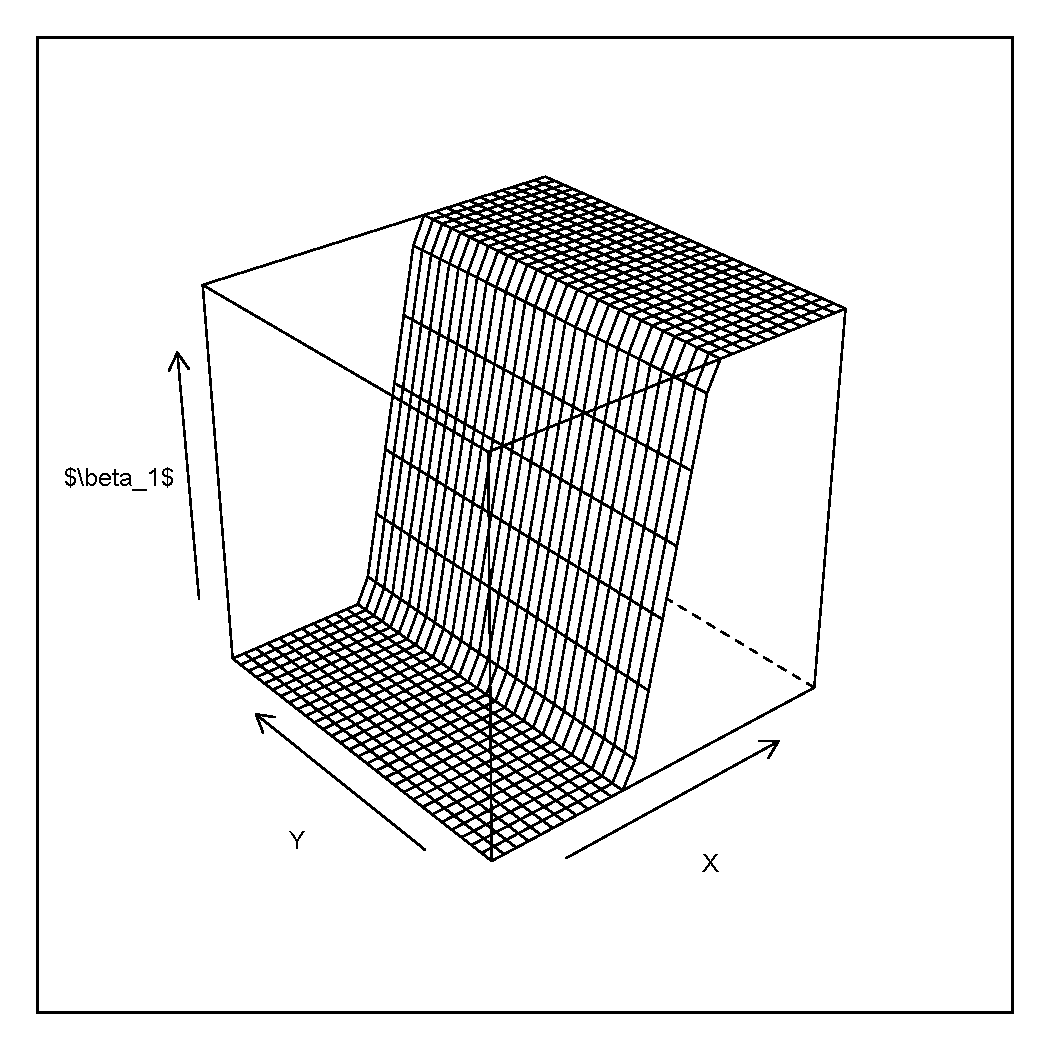
\includegraphics[width=0.3\textwidth]{../../figures/scratch/beta1-actual}}
	  \subfloat[]{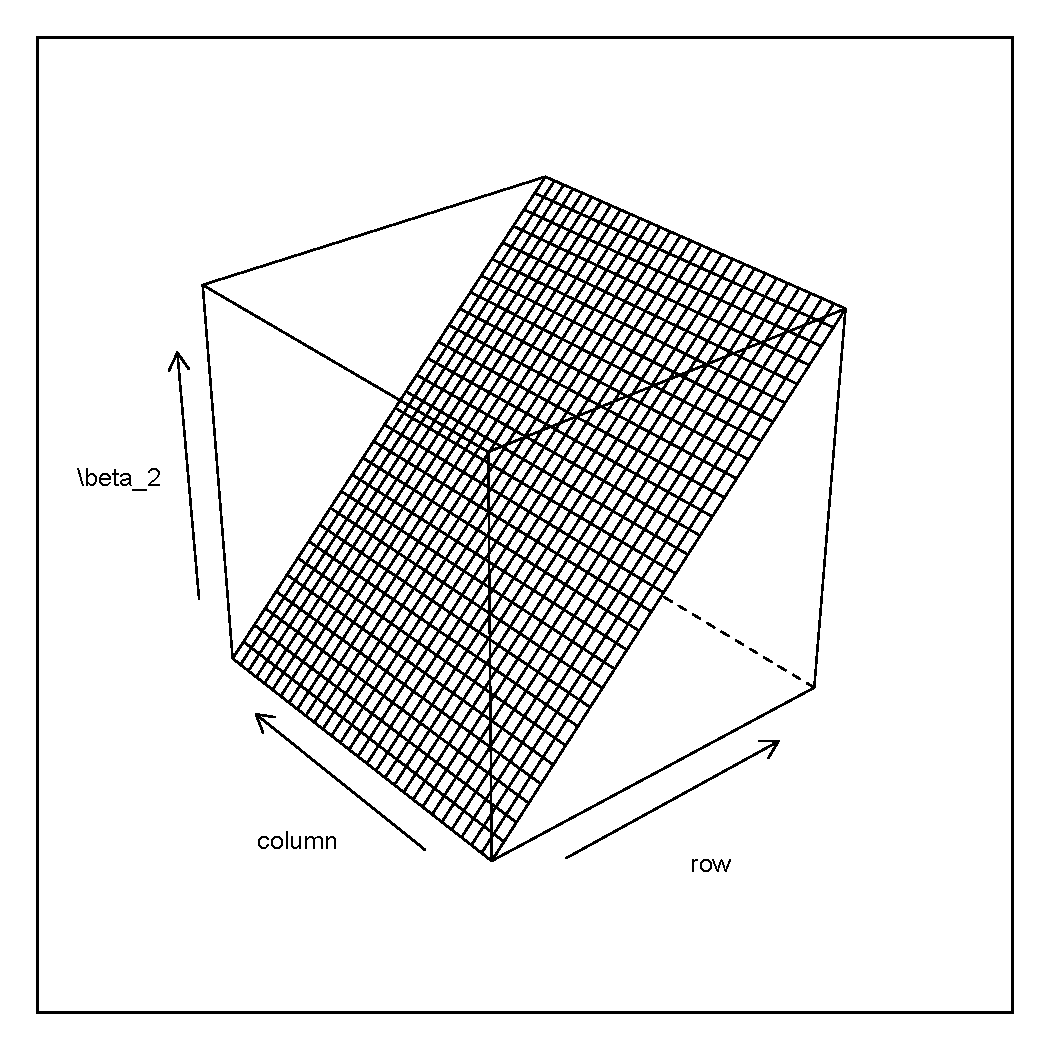
\includegraphics[width=0.3\textwidth]{../../figures/scratch/beta2-actual}}
	  \subfloat[]{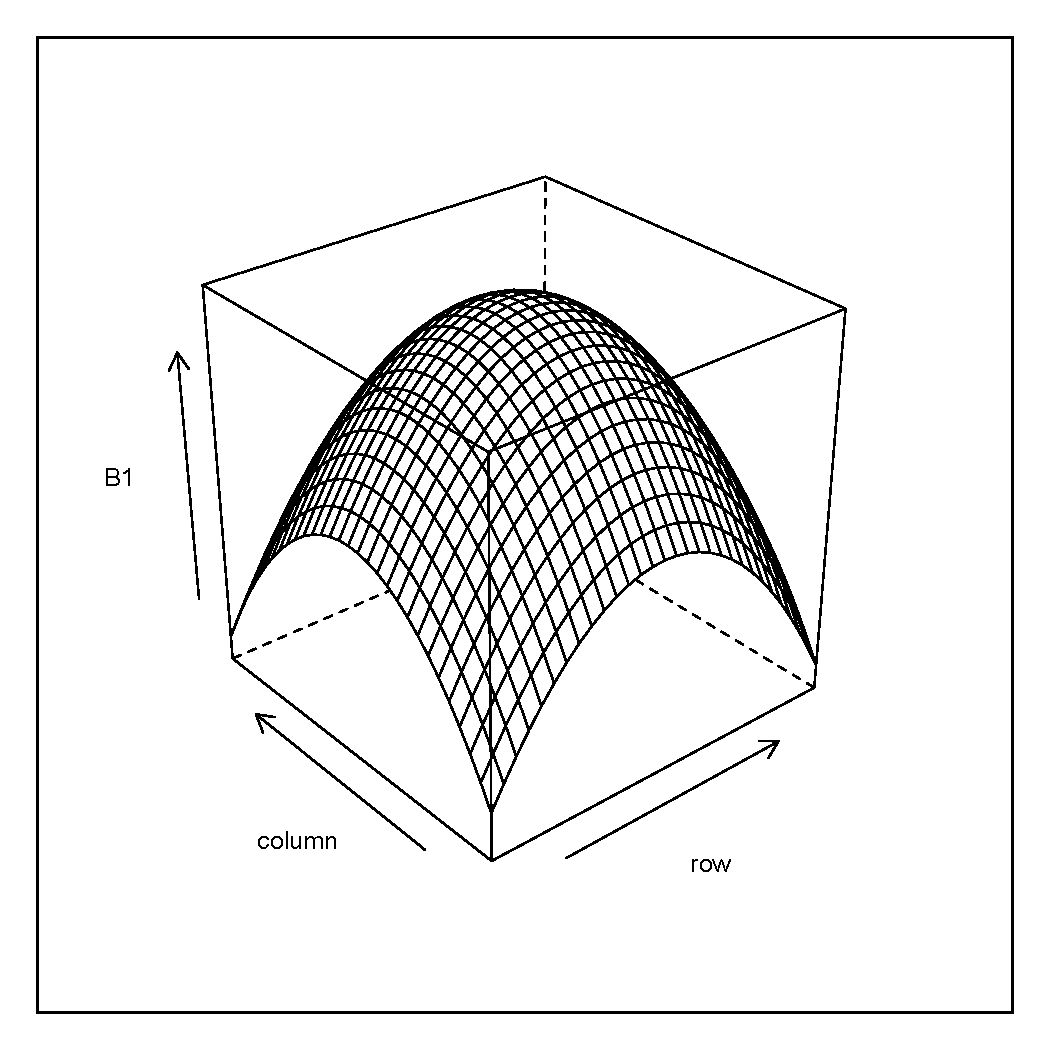
\includegraphics[width=0.3\textwidth]{../../figures/scratch/beta3-actual}}
        \end{center}
        \end{figure}

    \end{frame}
       
                    
    
    \begin{frame}{VCR estimation}
        \begin{itemize}
            \item VCR is a special case of a generalized additive model (GAM) \citep{Hastie:1986, Hastie:1990}
            \item Kernel-based methods: \cite{Hastie:1993b, Loader:1999}
            \item Spline-based methods: R implementation is the gam package \citep{Wood:2006} 
        \end{itemize}
    \end{frame}


    \begin{frame}{Kernel-based methods for estimation}
        \begin{itemize}
            \item Local likelihood, given book-length treatment in \cite{Loader:1999}
            \item Most literature puts the smoothing kernel on the same variable as the coefficient
            \item GWR: kernel is on location, coefficient on other covariates.
        \end{itemize}
    \end{frame}
	 

    \begin{frame}{Spline-based methods for estimation}
        \begin{itemize}
            \item Smoothing splines: a method of estimating a smooth function through data \citep{Wahba:1990}
            \item The smooth function is pieced together, pieces centered on each observation, with the requirement that the first two derivatives match up at the joints
            \item Model can be parameterized to get coefficient functions \citep{Hastie:1993a}
        \end{itemize}
    \end{frame}
    
    
    %\section{Spatial regression}
    %Spatial regression
    %\begin{frame}{Spatial Regression}
        %Geostatistical data is the name for observations of a continuous spatial process that are made at discrete locations. 
        %Clustering is a typical form of non-stationarity in spatial data. One way to analyze clustered data is to assume a constant underlying mean with random deviations that are clustered in space. This is the structure of an autoregressive model \citep{}. If the underlying mean is not constant but is given by a regression function with constant coefficients, then a conditionally autoregressive (CAR) model \citep{} is used to simultaneously estimate regression coefficients and clustering of the residuals.
    %\end{frame}


    \section{Geographically weighted regression}
    \begin{frame}{Geographically weighted regression (GWR)}
        \begin{itemize}
            \item Geographically-weighted regression \citep{Brundson:1998} is a kernel-based method of estimating spatial VCR models
            \item Main reference is the book \cite{Fotheringham:2002}     
        \end{itemize}
    \end{frame}
    


    \subsection{Local regression}
    %Local regression
    \begin{frame}{Local regression}
        \begin{itemize}
            \item Bias is known to be a problem in kernel smoothing \citep{Hastie:1993b}
        \end{itemize}

        \begin{figure}
        \begin{center}
	  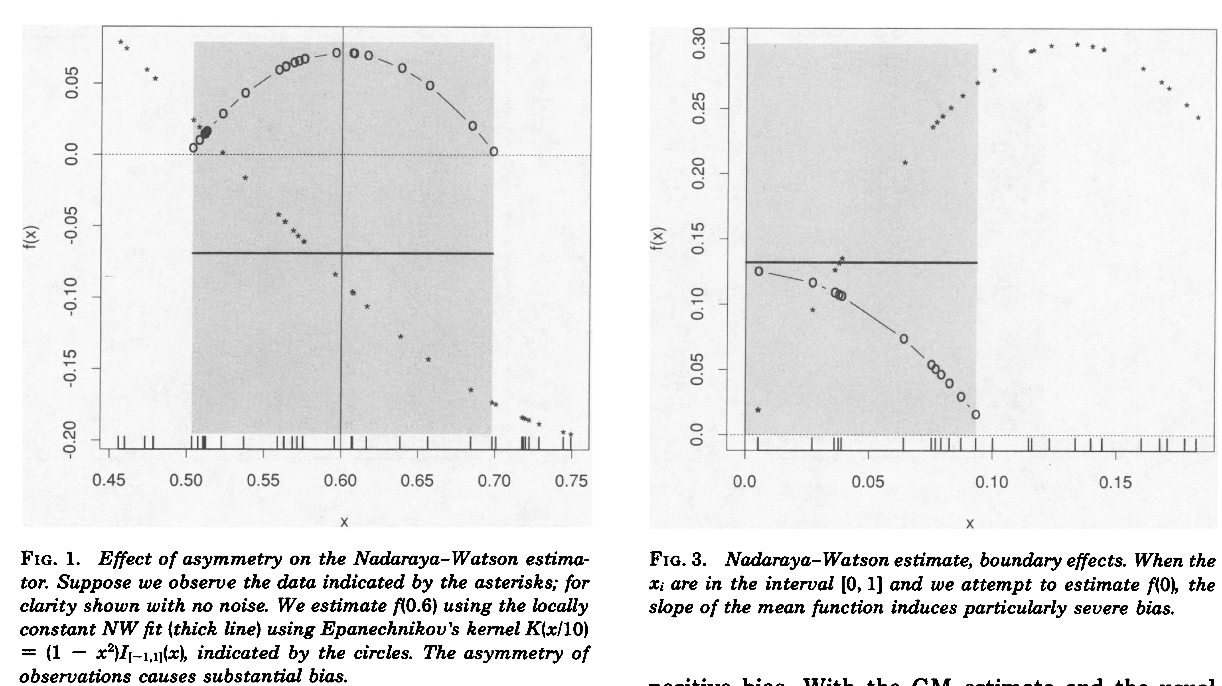
\includegraphics[width=0.8\textwidth]{../../figures/scratch/kernelbias}
        \end{center}
        \end{figure}
    \end{frame}
    
    
    %Local regression
    \begin{frame}{Local regression}      
        \begin{itemize}
            \item Local regression (locally linear fits) reduce bias
            \item Local regression introduced in GWR context by \cite{Wang:2008b}
        \end{itemize}  

        \begin{figure}
        \begin{center}
	  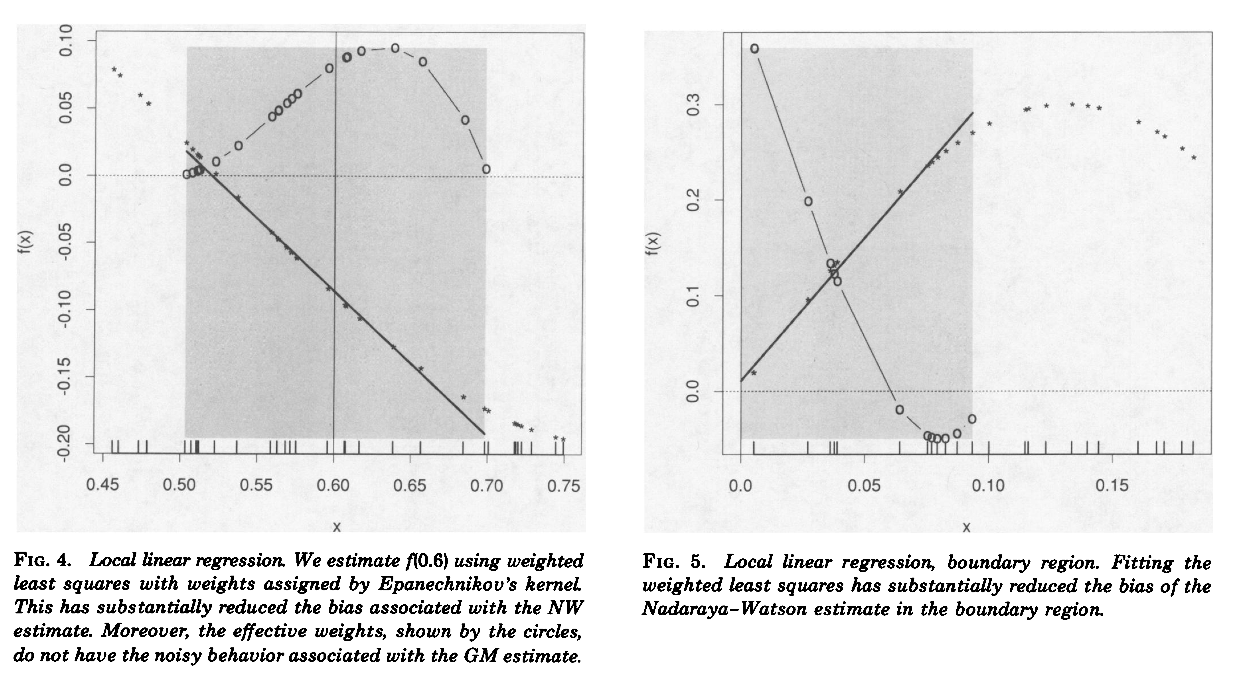
\includegraphics[width=0.8\textwidth]{../../figures/scratch/localregressionbias}
        \end{center}
        \end{figure}
    \end{frame}
    
    	


    \section{Variable selection for spatial VCR models}
    %Variable selection for spatial VCR models
    \begin{frame}{Variable selection for spatial VCR models}
        \begin{itemize}
            \item Global selection
            \item Local selection
        \end{itemize}
        %There is interest among practitioners of GWR not only in estimating the spatially-varying coefficient surface, but in doing variable selection to estimate which covariates are important predictors of the output variable, and in what regions they are important (citations?).
    \end{frame}
    

    \subsection{Global variable selection}
    %Global Variable selection
    \begin{frame}{Global variable selection}
        \begin{itemize}
            \item  \cite{Fan:1999} for response variables that belong to an exponential-family distribution (as in the generalized linear model)
            \item \cite{Wang:2008a} for models with repeated measurements.
        \end{itemize}
    \end{frame}


    \subsection{Local variable selection}
    %Local variable selection
    \begin{frame}{Local variable selection}
        \begin{itemize}
            \item \cite{Antoniadis:2012a} estimates the coefficient functions with P-splines, and then uses the nonnegative garrote of \cite{Breiman:1995} to do local variable selection by selecting P-spline bases.
            \item \cite{Wheeler:2009} uses the LASSO with a jackknife criterion that limits selection to observation locations.
        \end{itemize}
    \end{frame}

\section{References}
\bibliographystyle{chicago}
\bibliography{../../references/gwr}

\end{document}
